\documentclass[screen]{beamer}
% Angir foredragsholder, også en (valgfri) kortversjon i
% hakeparanteser først som kommer nederst på hver slide:
\author[Christian Chavez]{Christian Chavez}

\usepackage[T1]{fontenc}
\usepackage[utf8]{inputenc}
\usepackage{lmodern}

\usepackage{graphicx}
\usepackage{attrib}
\usepackage{amsmath}
\usepackage{amsfonts}
\usepackage{tikz-cd}

% Specify theme
%\usetheme{Madrid} %Theme that came with example
%\usetheme{Goettingen} %Theme that kvalsvik used
%\usetheme{Copenhagen}
% See http://goo.gl/Wxlyy for alternative themes

%\usetheme{ntnubokmaal}
%\usetheme{ntnunynorsk}
\usetheme{ntnuenglish}

% Specify base color
%\usecolortheme[named=OliveGreen]{structure}
% See http://goo.gl/p0Phn for alternative colors

% Specify other colors and options as required
%\setbeamercolor{alerted text}{fg=Maroon}
%\setbeamertemplate{items}[square]

% Angi tittelen, vi gir også en kortere variant som brukes nederst på
% hver slide:

\title[Compiler Offloading]{TDT24 Paper presentation}

% Denne kan du også bruke hvis det passer seg:
\subtitle{\textit{Offload Compiler Runtime for the
Intel\circledR Xeon Phi\texttrademark Coprocessor} \newline C.J. Newton, R.
Deodhar, S. Dmitriev, et al.; Intel 2013}

% Institusjon. Bruk gjerne disse slik det passer best med det du vil
% ha.  Valgfri kortversjon her også
\institute[IDI - NTNU]{Institutt for Datateknikk og Informasjonsvitenskap}
% Datoen blir også trykket på forsida.
%\date{13. juni 2005}
\date[November 2014]{\today} % Bruk denne hvis du ikke vil ha noe dato på forsida.

\begin{document}

% Siden NTNU-malen har en annen bakgrunn på forsida, må dette gjøres
% i en egen kommando, ikke på vanlig beamer-måte:
\ntnutitlepage

\begin{frame}{Outline}
    \tableofcontents
\end{frame}

\section{Introduction}

\begin{frame}{Motivation}
    \structure{What happens when you have a codebase containing millions of lines of code?}
    \pause
    \begin{center}
        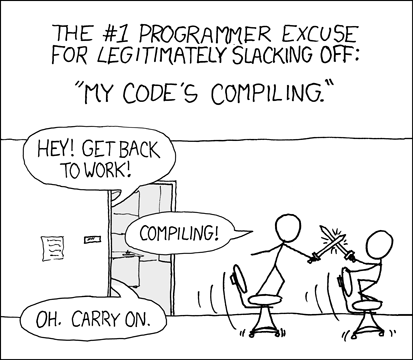
\includegraphics[width=0.5\linewidth]{compiling.png}
    \end{center}
\end{frame}

\section{Background: GPGPUs}

\begin{frame}{GPGPUs}
    So, how can \textit{GPGPUs} help?
    \begin{enumerate}[<+-| alert@+>]
        \item Split up and run sub-parts of the compilation \textbf{concurrently} with host (CPU)
        \item Run \textbf{computationally heavy} parts of the compiler algorithms, while the CPU works on the more serial ones.
    \end{enumerate}
\end{frame}

\section{Background: Xeon Phi}

\begin{frame}{Intel coprocessors}
    \structure{Intel wants to enter this market with the help of the \textbf{Xeon Phi} processor family}
    \pause
    \begin{itemize}
        \item Intended as a \textbf{competitor} against Nvidia CUDA GPGPUs in the HPC market
    \end{itemize}
\end{frame}

\begin{frame}{Xeon Phi drawbacks}
    Obvious \textit{drawbacks} with Xeon Phi (compared with the CUDA GPGPUs)
    \begin{enumerate}[<+-| alert@+>]
        \item Not as \textbf{mature} ecosystem/tools/environment
        \item Still requires a high degree of \textbf{computation to communication} to be beneficial to run on the Phi instead of the CPU
        \item Still new and relatively untested/unused wrt. compilers
        \item Being Intel, everything is ``canned'' (not open source)
    \end{enumerate}
\end{frame}

\begin{frame}{Xeon Phi benefits}
    Obvious \textit{benefits} with Xeon Phi (compared with the CUDA GPGPUs)
    \begin{enumerate}[<+-| alert@+>]
        \item The architecture supports regular Intel CPU instructions\footnote{Not confirmed exactly how much}
        \begin{itemize}[<+-| alert@+>]
            \item The Xeon Phi does not require its own codebase for being run.
        \end{itemize}
    \end{enumerate}
\end{frame}

\section{Runtime Offloading: Tools}

\begin{frame}{Runtime offloading tools}
    The papers focus is on the following tools:
    \begin{itemize}[<+-| alert@+>]
        \item Intel Manycore Platform Software Stack (MPSS)
        \begin{itemize}
            \item Intel Coprocessor Offload Infrastructure (COI)
        \end{itemize}
        \item COI utilizes:
        \begin{itemize}[<+-| alert@+>]
            \item Library calls
            \item Language pragmas
            \item Language keywords
            \item A FIFO command queue (dataobject: COIPipeline)
        \end{itemize}
        \item OpenMP
    \end{itemize}
\end{frame}

\section{Runtime Offloading: Application tests}

\begin{frame}{Platform specifications}
    Test platform specifications:
    \begin{center}
        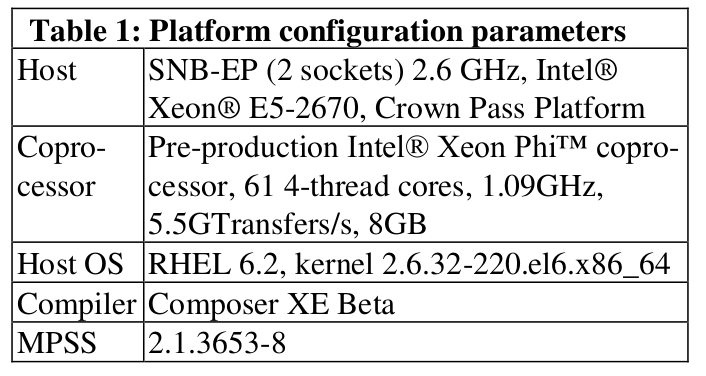
\includegraphics[width=0.8\linewidth]{table1.png}
    \end{center}
\end{frame}

\begin{frame}
    Two sets of tests:
    \begin{enumerate}[<+-| alert@+>]
        \item A test spanning a variety of application domains, coming from customers.
        \begin{itemize}
            \item Hence, some names are occluded in deference to customers.
            \item The tests are meaningfully representative to said customers.
        \end{itemize}
        \item An array of benchmarks from Scalable HeterOgeneous Computing (\textit{SHOC}) benchmarks suite.
        \begin{itemize}
            \item Only used tests that were not exclusive to OpenCL and CUDA
            \item Only used tests that have both offload and native versions
            \item Results were measured by Intel in August 2012.
            \item The benchmark application \textit{Triad} was also added, even though it has no native version
        \end{itemize}
    \end{enumerate}
\end{frame}

\section{Runtime Offloading: Test results}

\begin{frame}{Customer tests results}
    \begin{center}
        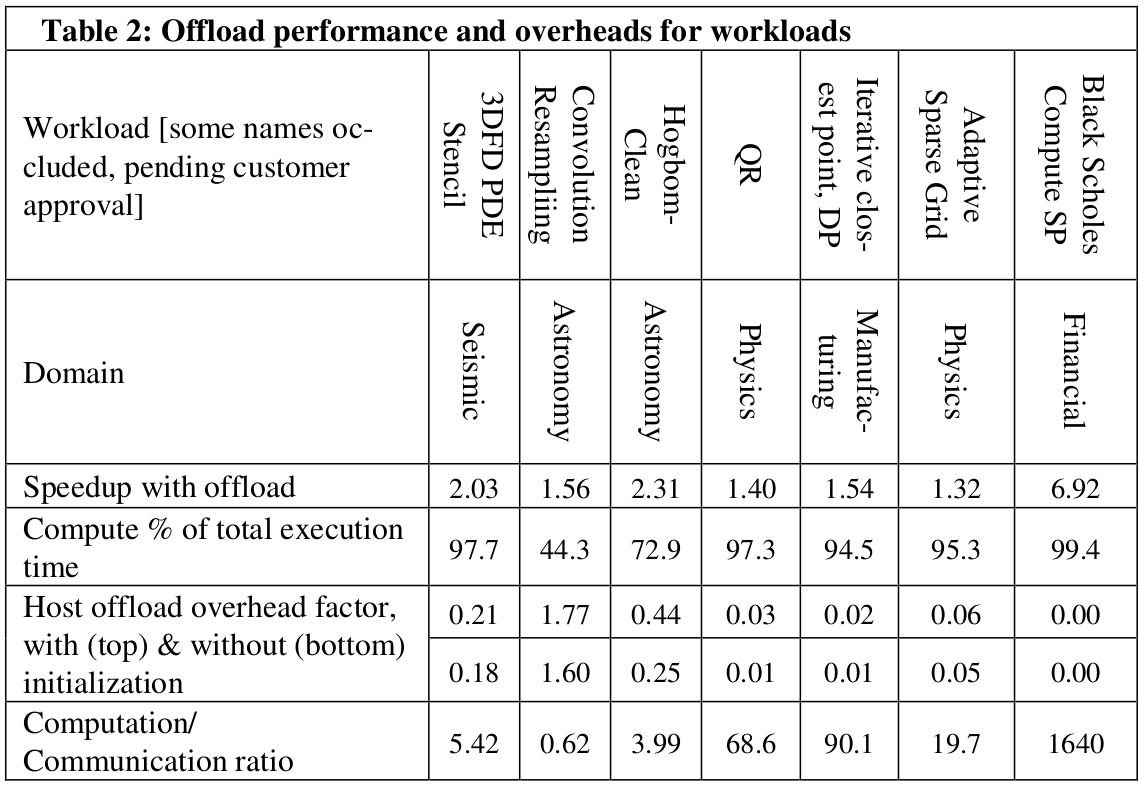
\includegraphics[width=0.65\linewidth]{table2.png}
    \end{center}
\end{frame}

\begin{frame}{SHOC tests results}
    \begin{center}
        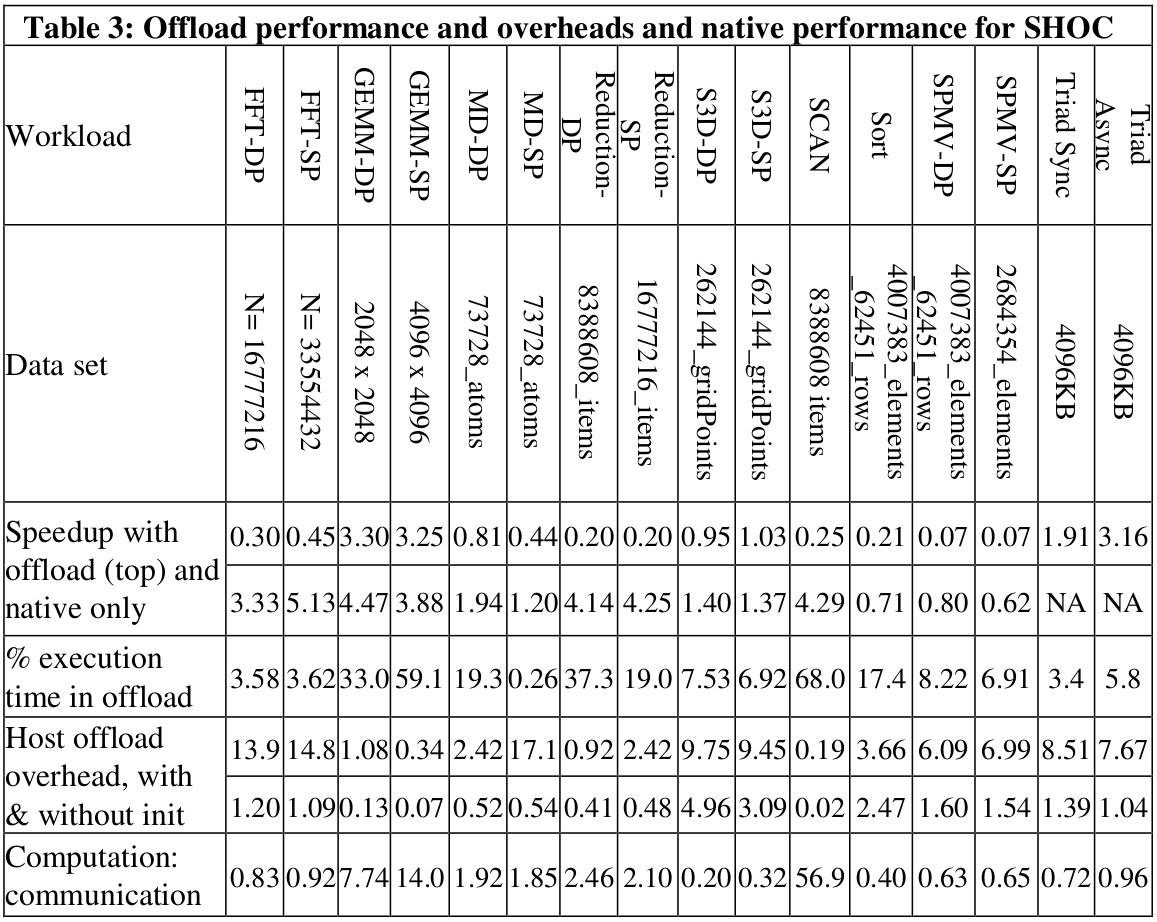
\includegraphics[width=0.6\linewidth]{table3.png}
    \end{center}
\end{frame}

\begin{frame}{Speedups 1/2}
    \begin{itemize}[<+-| alert@+>]
        \item Computation to communication ratio varied from 0.62 to 1640
        \begin{enumerate}[<+-| alert@+>]
            \item But it was generally over 4, except for the convolution case.
            \item The convolution case scaling across threads and SIMD elements on the coprocessor allowed the computation speedup to outweigh the overheads
        \end{enumerate}
        \item Data movement overhead varied from neglegible to 1.77x the computation time
        \item Black Scholes was the big performance winner, with a 6.92x speedup of the dual-socket SandyBridge
        \item SHOC shows no correlation between speedup and computation to communication.
        \begin{itemize}
            \item Paper lists this as potential future work. \\
                ``Broader investigation is needed on that''
        \end{itemize}
    \end{itemize}
\end{frame}

\begin{frame}{Speedups 2/2}
    ``No single factor determines offload performance''
    \begin{itemize}[<+-| alert@+>]
        \item Data movement overhead varied from neglegible to 1.77x the computation time
    \end{itemize}
    Offload speedups are most correlated with the following:
    \begin{enumerate}[<+-| alert@+>]
        \item Inverse of offload overheads
        \item \% of execution time in offload (which includes coprocessor invocation and data movement)
        \item Native performance (when there is no execution on the host at all)
    \end{enumerate}
\end{frame}

\section{Conclusion}

\begin{frame}{Conclusion}
    \begin{itemize}
        \item The Xeon Phi in conjunction with the platform used in the paper showed benchmark application speedups from 1.3x to 6.9 on ``customer-relevant'' examples spanning different application domains
        \item Offload is not always profitable, as SHOC showed
        \item Inhibitions or enhancements of speedup this paper has explored:
        \begin{enumerate}
            \item When response time is of concern, there must be a speedup from native execution on only the coprocessor, relative to the execution on the host
            \item Ratio of computation to communication must be generally high
            \item Offload runtime overheads must be small relative to computation
        \end{enumerate}
    \end{itemize}
\end{frame}

\begin{frame}{Sources}
    \begin{itemize}
        \item \textit{Offload Compiler Runtime for the Intel\circledR  Xeon Phi\texttrademark  Coprocessor}, Newton, R.
Deodhar, S. Dmitriev, et al.\footnote{\url{https://software.intel.com/sites/default/files/article/366893/offload-runtime-for-the-intelr-xeon-phitm-coprocessor.pdf}}
        \item Randall Munroe, xkcd\footnote{\url{http://xkcd.com/303/}}
    \end{itemize}
\end{frame}

\end{document}
